\begin{figure}[t!]
\centering
\subfigure[]{
% 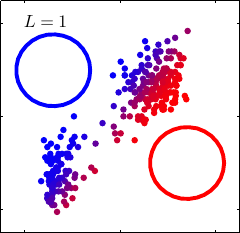
\includegraphics[width=0.40\columnwidth]{resources/em/EM1.png}
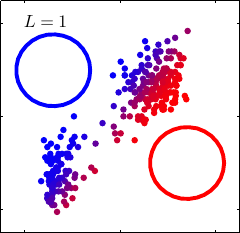
\includegraphics[width=0.21\textwidth]{resources/em/EM1.png}
}\quad
\subfigure[]{
% 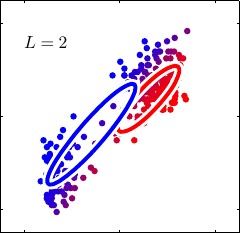
\includegraphics[width=0.40\columnwidth]{resources/em/EM2.png}
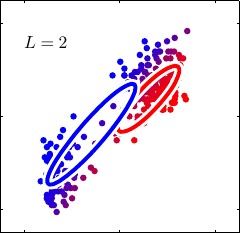
\includegraphics[width=0.21\textwidth]{resources/em/EM2.png}
}\quad
\subfigure[]{
% 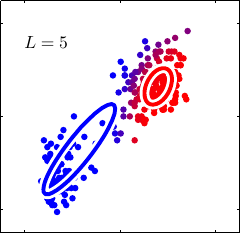
\includegraphics[width=0.40\columnwidth]{resources/em/EM3.png}
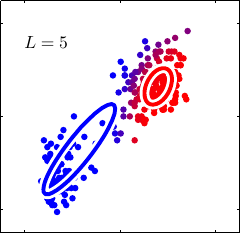
\includegraphics[width=0.21\textwidth]{resources/em/EM3.png}
}\quad
\subfigure[]{
% 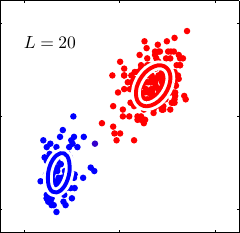
\includegraphics[width=0.40\columnwidth]{resources/em/EM4.png}
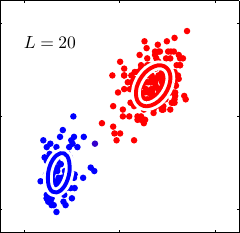
\includegraphics[width=0.21\textwidth]{resources/em/EM4.png}
}\quad
\caption{
Visualization of Expectation-Maximization algorithm \cite{bishopPatternRecognitionMachine2006}.
(a) Clusters are randomly initialized. 
(b) Cluster centers are updated according to the initial assignment (M step).
(c), (d) Expectation and Maximization steps are repeated until convergence.
}
\label{fig:em}
\end{figure}    